\documentclass[border=5pt]{standalone}
\usepackage{tikz}
\usetikzlibrary{arrows.meta}
\begin{document}
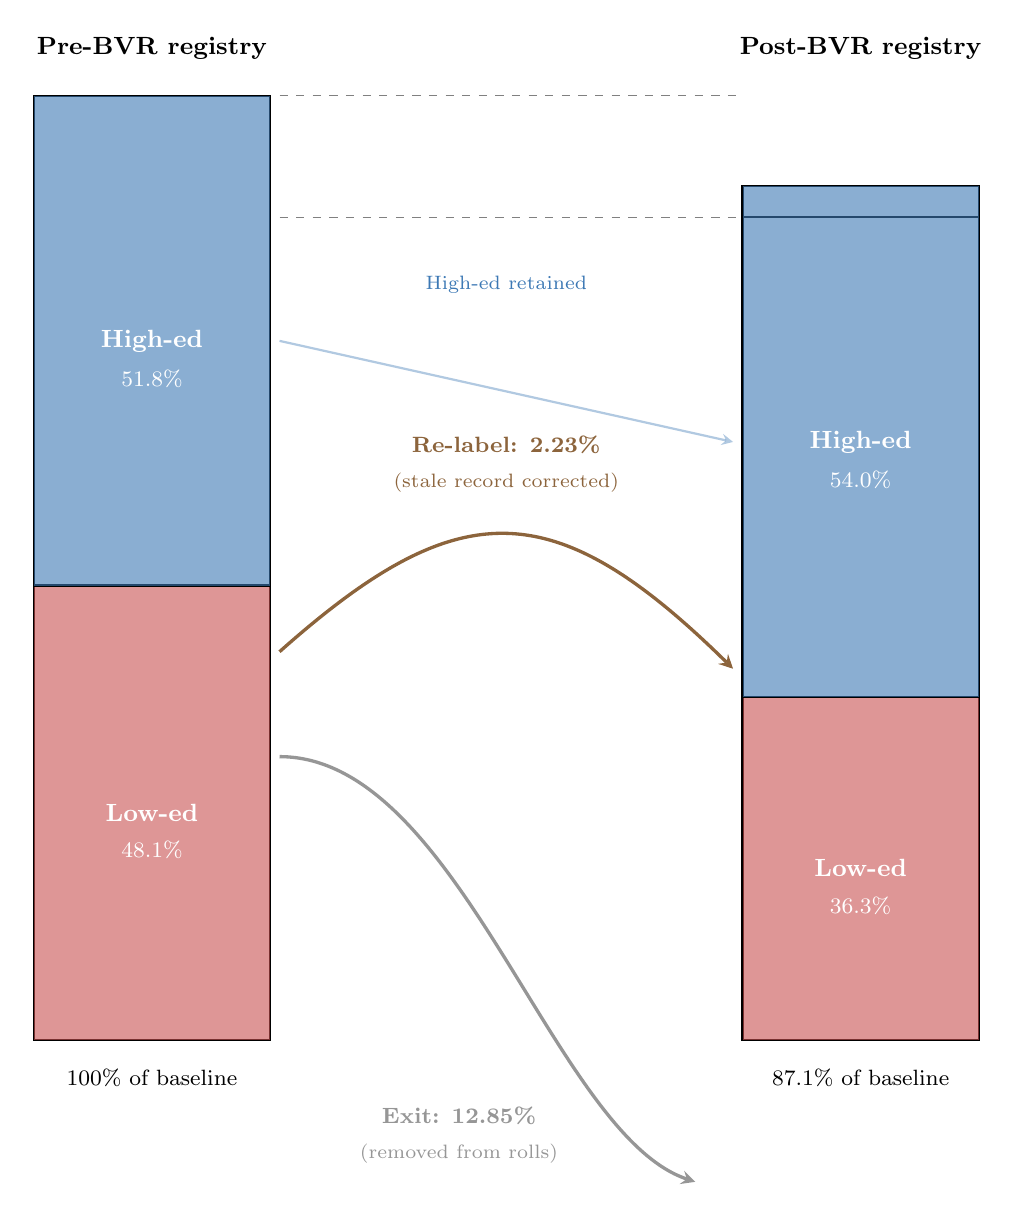
\begin{tikzpicture}[scale=1.2, >=stealth]

\definecolor{loweducolor}{RGB}{200, 80, 80}
\definecolor{higheducolor}{RGB}{60, 120, 180}
\definecolor{relabelcolor}{RGB}{140, 100, 60}
\definecolor{exitcolor}{RGB}{150, 150, 150}

\draw[thick] (0, 0) rectangle (2.5, 9.99);
\fill[loweducolor, opacity=0.6] (0, 0) rectangle (2.5, 4.81);
\node[white, font=\small\bfseries] at (1.25, 2.41) {Low-ed};
\node[white, font=\footnotesize] at (1.25, 2.01) {48.1\%};

\draw[thick] (0, 4.81) rectangle (2.5, 9.99);
\fill[higheducolor, opacity=0.6] (0, 4.81) rectangle (2.5, 9.99);
\node[white, font=\small\bfseries] at (1.25, 7.40) {High-ed};
\node[white, font=\footnotesize] at (1.25, 7.00) {51.8\%};

\node[font=\small\bfseries] at (1.25, 10.5) {Pre-BVR registry};
\node[font=\footnotesize] at (1.25, -0.4) {100\% of baseline};

\draw[thick] (7.5, 0) rectangle (10.0, 8.71);
\fill[loweducolor, opacity=0.6] (7.5, 0) rectangle (10.0, 3.63);
\node[white, font=\small\bfseries] at (8.75, 1.82) {Low-ed};
\node[white, font=\footnotesize] at (8.75, 1.42) {36.3\%};

\draw[thick] (7.5, 3.63) rectangle (10.0, 9.04);
\fill[higheducolor, opacity=0.6] (7.5, 3.63) rectangle (10.0, 9.04);
\node[white, font=\small\bfseries] at (8.75, 6.33) {High-ed};
\node[white, font=\footnotesize] at (8.75, 5.93) {54.0\%};

\node[font=\small\bfseries] at (8.75, 10.5) {Post-BVR registry};
\node[font=\footnotesize] at (8.75, -0.4) {87.1\% of baseline};

\draw[dashed, thin, gray] (2.6, 10.0) -- (7.5, 10.0);
\draw[dashed, thin, gray] (2.6, 8.71) -- (7.5, 8.71);

\draw[->, very thick, exitcolor] (2.6, 3.0) .. controls (4.5, 3.0) and (5.5, -1.0) .. (7.0, -1.5);
\node[exitcolor, font=\footnotesize\bfseries] at (4.5, -0.8) {Exit: 12.85\%};
\node[exitcolor, font=\scriptsize] at (4.5, -1.2) {(removed from rolls)};

\draw[->, very thick, relabelcolor] (2.6, 4.11) .. controls (4.5, 5.8) and (5.5, 5.8) .. (7.4, 3.93);
\node[relabelcolor, font=\footnotesize\bfseries] at (5.0, 6.3) {Re-label: 2.23\%};
\node[relabelcolor, font=\scriptsize] at (5.0, 5.9) {(stale record corrected)};

\draw[->, thick, higheducolor, opacity=0.4] (2.6, 7.40) -- (7.4, 6.33);
\node[higheducolor, font=\scriptsize] at (5.0, 8.0) {High-ed retained};

\end{tikzpicture}
\end{document}
